\section{Adressierbare RGB-LEDs als Anzeigeelement}
Die \gls{ws2812b} ist eine integrierte \gls{rgb}-\gls{led} mit eingebauter Steuerelektronik. 
Sie kombiniert eine Lichtquelle und eine digitale Ansteuerlogik in einem gemeinsamen Gehäuse der Bauform 5050. 
Dadurch entfällt die Notwendigkeit externer Treiberschaltungen für einzelne \gls{led}s, was den Schaltungsaufwand reduziert und die Integration vereinfacht~\cite{Worldsemi2013}.

Ein wesentliches Merkmal der \gls{ws2812b} ist die serielle Ansteuerung über eine einzelne Datenleitung. 
Die Kommunikation erfolgt über ein digitales Protokoll, bei dem die Daten bitweise übertragen werden. 
Jede \gls{led} empfängt dabei einen Datenstrom, verarbeitet die ersten 24 Bit zur eigenen Darstellung und leitet die verbleibenden Daten an nachfolgende \gls{led}s weiter. 
Dieses Prinzip ermöglicht die Realisierung langer \gls{led}-Ketten mit minimalem Verdrahtungsaufwand~\cite{Worldsemi2013}. 

Die Farbdarstellung basiert auf drei integrierten Leuchtdioden für die Grundfarben Rot, Grün und Blau. 
Für jede dieser Komponenten stehen 8 Bit zur Verfügung, wodurch sich insgesamt 24 Bit pro \gls{led} ergeben. 
Dies ermöglicht die Darstellung von bis zu 16.777.216 verschiedenen Farbwerten. 
Die Datenübertragung erfolgt in einer fest definierten Reihenfolge der Farbkanäle, wodurch eine konsistente Farbwiedergabe gewährleistet wird.
Die Versorgung der \gls{ws2812b} erfolgt mit +5V. 
Jede \gls{led} enthält eine interne Konstantstromsteuerung, wodurch eine gleichmäßige Helligkeit unabhängig von Versorgungsschwankungen erreicht wird~\cite{Worldsemi2013}. 

Ein weiterer Vorteil liegt in der Möglichkeit zur einfachen Kaskadierung (vgl. Abb.~\ref{fig:KaskadeLED}).
Mehrere \gls{led}s können direkt hintereinander geschaltet werden, wobei der Ausgang einer \gls{led} mit dem Eingang der nächsten verbunden wird. 
Die maximale Anzahl der kaskadierbaren \gls{led}s hängt primär von der Datenrate und der gewünschten Aktualisierungsfrequenz ab. 
Bei typischen Anwendungen können mehrere hundert bis über 1000 \gls{led}s ohne zusätzliche Signalverstärkung betrieben werden~\cite{Worldsemi2013}.

\begin{figure}[H]
	\centering
	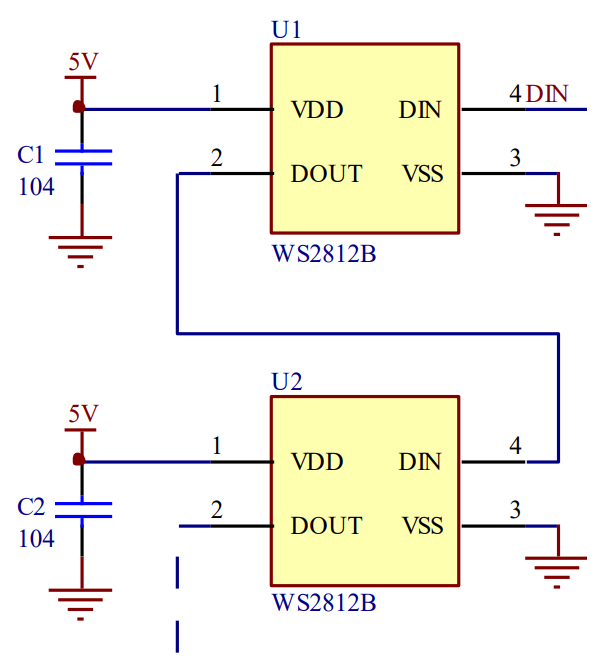
\includegraphics[width=0.5\linewidth]{inhalt/bilder/KaskadeLED.png}
	\caption{Schaltbild zur Kaskadierung von \gls{ws2812b} \gls{led}s mit einer Versorgungsspannung von +5V. Mit VDD als Versorgungsspannung, DIN als Datensignal Eingang, DOUT als Datensignal Ausgang und VSS als als Ground~\cite{Worldsemi2013}.}
	\label{fig:KaskadeLED}
\end{figure}

Für Anwendungen wie WordClocks ergibt sich aus diesen Eigenschaften eine geeignete Architektur. 
Die einzelne Adressierbarkeit ermöglicht die gezielte Darstellung wobei die geringe Anzahl benötigter Steuerleitungen in einem geringen Verdrahtungsaufwand resultiert. 
Gleichzeitig erlaubt die hohe Farbauflösung eine flexible Gestaltung der Anzeige, beispielsweise zur Differenzierung von Funktionen oder Zuständen~\cite{Worldsemi2013}.